\newpage
\usecaseautenticato{Effettua \textit{Logout}}
\label{usecase:Effettua Logout}

\begin{figure}[h]
	\centering
	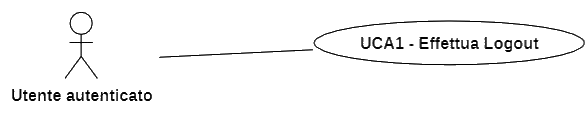
\includegraphics[width=0.8\textwidth]{./uml/UCA1.png} 
	\caption{Effettua \textit{Logout}}
	\label{fig:UCA1}
  \end{figure}

\begin{itemize}
	\item \textbf{Attore principale:} Utente autenticato.

	\item \textbf{Precondizioni:}
	\begin{itemize}
        \item L'Utente ha eseguito correttamente l'accesso al Sistema come Utente base(vedi \autoref{usecase:Effettua accesso}).
        \item L'utente deve trovarsi nella sua Area personale$^G$.
    \end{itemize}

	\item \textbf{Postcondizione:} L'utente esegue con successo il \textit{logout}.

	\item \textbf{Scenario principale:}
	      \begin{enumerate}
		      \item L'Utente autenticato naviga nella sezione Area personale$^G$.
		      \item L'Utente autenticato avvia la procedura di \textit{logout}.
              \item Il Sistema disconnette l'Utente dal suo \textit{account} e lo reindirizza alla \textit{Home} del sito, identificandolo come Utente generico.
	      \end{enumerate}
\end{itemize}
